\documentclass[10pt]{article}
\usepackage[preprint]{tmlr-style-file-main/tmlr-style-file-main/tmlr}
\usepackage[T1]{fontenc}
\usepackage{lmodern}
\usepackage{microtype}
\usepackage{amsmath}
\usepackage{tikz}
\usepackage{circuitikz}
\usepackage{float}
\usepackage{graphicx}
\usepackage{tabularx}
\usepackage{xcolor}
\usetikzlibrary{positioning}
\usepackage{booktabs}
\usepackage{longtable}
\usepackage{array}
\usepackage{enumitem}
\usepackage[hidelinks,hypertexnames=false]{hyperref}

\setlist[itemize]{leftmargin=1.6em}
\setlist[enumerate]{leftmargin=1.8em}
\vbadness=10000
\setlength{\floatsep}{8pt plus 2pt minus 2pt}
\setlength{\textfloatsep}{10pt plus 2pt minus 2pt}
\setlength{\intextsep}{8pt plus 2pt minus 2pt}

\newcolumntype{Y}{>{\raggedright\arraybackslash}X}

\def\month{03}
\def\year{2026}
\def\openreview{\url{https://openreview.net/forum?id=XXXX}}

\begin{document}

\title{Machine Learning Assignment Report\\
\large Two-Player Sushi Go Reinforcement Learning System}
\author{Chenhe Yuan, Student Number: 22003915 \\ Guanfang Lai Student Number: 21010826\\ Simon Zhu, Student Number: 22020163 \\ Xander Mills, Student Number: 22078470}
\date{\today}
\maketitle

\begin{abstract}
This report presents a two-player Sushi Go reinforcement learning system implemented in Python. The project emphasizes rule correctness, reproducibility, and trainability, and combines a deterministic game simulator, baseline opponents, policy optimization, and statistical evaluation in one pipeline. The final system targets the repository's current three-round Sushi Go variant, including Pudding and Chopsticks, rather than a simpler one-round draft-only benchmark. The selected model design uses MaskablePPO with a fixed-length MLP state representation and an explicit legal-action mask so that training remains stable despite sparse terminal rewards and dynamically constrained legal actions. In addition to describing the implementation, this merged report adds concrete experimental evidence, including baseline controls, a fresh 1,000,000-step curriculum run, an ablation study comparing curriculum against single-opponent training regimes, and qualitative examples from the LLM coaching interface. The reproduced checkpoint \texttt{repro\_curriculum\_1m} achieves a deterministic 96.6\% win rate against a random opponent and 95.7\% against the heuristic baseline over 1000 episodes. The ablation shows that training against random opponents only drops the win rate against the heuristic to 0.866, confirming that curriculum training is the key driver of generalisation across opponent types.
\end{abstract}

\section{Introduction}

This project develops a two-player Sushi Go reinforcement learning system in Python, with the objective of producing a rule-correct, reproducible, and trainable game environment for policy learning and evaluation. The implemented system combines a deterministic game simulator, baseline opponents, policy training, and statistical evaluation into one research-oriented pipeline. The project frames the game as a controlled sequential decision-making benchmark in which environment dynamics, scoring, and reward signals are explicitly defined, auditable, and testable.

The implementation targets a three-round, two-player variant of Sushi Go that includes Pudding and Chopsticks mechanics. Each round deals ten cards per player from a fixed deck, both players act simultaneously, and the remaining hands are passed after each turn. Round-level decisions therefore interact with delayed incentives such as maki races within the round, Wasabi setup value, and end-of-game Pudding scoring across all three rounds. The software architecture separates pure game logic from environment transition logic, which improves both correctness and auditability. In practice, this design supports repeatable reinforcement learning experiments under fixed seeds, stable comparison against baseline policies, and consistent evaluation of model performance through win rates and score differentials.

The report has two goals. First, it documents the current repository in a way that is faithful to the code. Second, it turns the project from an implementation description into a finished experimental report by combining the original implementation-focused write-up with fresh quantitative evidence, detailed baseline explanations, and grounded LLM interaction examples.

\section{Game Rules}

\subsection{Game Flow}

The game is played by two players over three rounds, with each player receiving ten cards at the beginning of each round from a shuffled fixed deck composition. On each turn, both players choose actions simultaneously, the selected cards are resolved in play order, and then the remaining hands are exchanged between players. This cycle continues until all ten turns in the round are completed. At the end of each round, the played cards are scored, round piles are cleared, and a new round begins until the third round is finished. After the final round, end-of-game Pudding scoring is applied and the episode terminates.

\subsection{Scoring Logic}

Scoring follows the repository ruleset for Tempura, Sashimi, Dumpling, Nigiri, Wasabi, Maki, Pudding, and Chopsticks. Tempura scores in pairs, Sashimi scores in triples, and Dumpling uses capped progressive scoring. Nigiri contributes base value, while Wasabi triples only the next Nigiri played after Wasabi appears; it does not retroactively affect earlier Nigiri. Maki scoring is comparative within a round: in two-player play, a tie for first splits first-place value. Pudding is handled differently from round cards because it is accumulated across all rounds and scored only once at game end. In this implementation, the player with more Pudding receives a bonus, while the player with fewer Pudding does not receive a negative penalty.

For clarity, the main card-category scoring rules are:
\begin{itemize}
  \item Tempura scores 5 points per pair.
  \item Sashimi scores 10 points per triple.
  \item Dumpling uses the capped progression \(0,1,3,6,10,15\).
  \item Nigiri scores according to face value unless multiplied by Wasabi.
  \item Wasabi triples only the next later Nigiri in play order.
  \item Maki is scored comparatively within each round.
  \item Pudding is scored once after the third round.
\end{itemize}

\subsection{Reward Design}

From a reinforcement learning perspective, reward shaping is intentionally minimal. Intermediate rewards are zero during the episode, and only the terminal reward is used, defined as the final score difference between the learning agent and the opponent:
\[
r_{\text{terminal}} = \texttt{my\_score} - \texttt{opp\_score}.
\]
This keeps optimization aligned with the actual game objective and avoids introducing artificial incentives that distort play quality. In particular, it prevents the policy from over-valuing locally attractive actions that might harm end-of-round maki outcomes or end-of-game pudding advantage.

\section{Task Characteristics and Model Design Rationale}

This task is a constrained sequential decision problem with combinational actions, hidden opponent intent, and delayed reward assignment. The Chopsticks mechanic makes the legal action set state-dependent, and the three-round format with end-of-game Pudding scoring means that many strategically important decisions are rewarded only at the end of the episode. Because of this structure, the core modelling question is not only whether the agent can optimize returns, but whether it can do so reliably under a dynamically constrained action space and sparse terminal feedback.

For this reason, the project adopts a MaskablePPO actor-critic model with an MLP policy over a fixed-size feature vector and a separate legal-action mask. Compared with unmasked policy-gradient or value-based alternatives, MaskablePPO directly enforces action legality during sampling, which removes a major source of instability in games where many indices are invalid at each turn. PPO is selected because its clipped objective and advantage-based updates are generally robust under sparse rewards and medium-horizon episodes, while still being practical to train and tune in small-to-medium environments. The MLP architecture is preferred over recurrent or transformer policies because the environment is represented by an explicit, fixed-length summary that already encodes the information needed for decision making, making heavier sequence models unnecessary at this stage.

The training setup further uses random and heuristic opponents, with optional curriculum mixing, to reduce overfitting to a single behaviour profile and to improve policy robustness. Overall, this model design balances correctness, learning stability, and experimental practicality, which is why it is a better fit for this project than more complex or less constrained alternatives.

\section{Requirements and Technical Stack}

The system is designed around a modern Python reinforcement learning stack with an emphasis on deterministic simulation, masked action selection, and experiment reproducibility. The environment layer is implemented with Gymnasium-compatible interfaces so that training algorithms can interact with the game through standard \texttt{reset} and \texttt{step} transitions. Numerical representation, state encoding, masking logic, and stochastic control are handled through NumPy. Policy optimization is implemented with Stable-Baselines3 and SB3-Contrib, specifically using MaskablePPO to ensure invalid actions are excluded during policy sampling. Testing and regression validation rely on PyTest, while plotting and result analysis are supported by Matplotlib.

A key technical requirement in this project is consistency between formal rules and runtime behaviour. To satisfy that requirement, card definitions and scoring are isolated in a pure rules module, while turn resolution and multi-round progression are implemented in the environment module. This separation allows direct unit-level validation of scoring logic and independent integration-level validation of episode dynamics. Another requirement is reproducibility for research use: randomization is centralized through seeded generators so that identical seeds and action sequences reproduce identical trajectories.

The stack is therefore selected for methodological control. Gymnasium enforces interface discipline across training and evaluation; NumPy ensures transparent, deterministic state handling; and MaskablePPO resolves the constrained action problem that would otherwise require custom sampling logic or penalty-based workarounds. The result is a pipeline where rules, environment dynamics, and policy optimization are independently verifiable and collectively coherent, which is the baseline requirement for a credible RL study on a non-trivial game environment.

\begin{table}[ht]
\centering
\begin{tabularx}{\textwidth}{@{}lY@{}}
\toprule
\textbf{Component} & \textbf{Purpose in the Project} \\
\midrule
Gymnasium & Standard interface for environment transitions and algorithm integration. \\
NumPy & Deterministic numerical operations, state encoding, and random-seed control. \\
Stable-Baselines3 + SB3-Contrib & Policy optimization with \texttt{MaskablePPO} and legal-action masking. \\
PyTest & Unit and regression validation for rules and episode dynamics. \\
Matplotlib & Plotting and analysis of evaluation outcomes. \\
\bottomrule
\end{tabularx}
\caption{Technical stack summary.}
\end{table}

\section{Implementation}

\subsection{System Architecture Overview}

The implementation is organized into modular components that separate game logic, environment dynamics, agent policies, and training infrastructure. This separation ensures that rules can be validated independently, environment behavior can be tested in isolation, and training experiments can be reproduced deterministically.

% \begin{figure}[!ht]
% \centering
% \resizebox{0.8\textwidth}{!}{%
% \begin{circuitikz}
% \tikzstyle{every node}=[font=\small, align=center, text width=2.1cm]

% \draw[fill=red!15, thick] (2.5,14.125) rectangle (5,12.875);
% \node at (3.75,13.5) {\texttt{train.py}\\training};

% \draw[fill=red!15, thick] (10,14.125) rectangle (12.5,12.875);
% \node at (11.25,13.5) {\texttt{eval.py}\\evaluation};

% \draw[fill=yellow!15, thick] (6.25,11.625) rectangle (8.75,10.375);
% \node at (7.5,11) {\texttt{agents/}\\policies};

% \draw[fill=green!15, thick] (6.25,9.125) rectangle (8.75,7.875);
% \node at (7.5,8.5) {\texttt{env.py}\\environment};

% \draw[fill=blue!15, thick] (6.25,6.625) rectangle (8.75,5.375);
% \node at (7.5,6) {\texttt{rules.py}\\scoring logic};

% \draw[-{Stealth[scale=1.5]}, very thick] (7.125,11.625) -- (5,12.875);
% \draw[-{Stealth[scale=1.5]}, very thick] (7.875,11.625) -- (10,12.875);
% \draw[-{Stealth[scale=1.5]}, very thick] (7.5,9.125) -- (7.5,10.375);
% \draw[-{Stealth[scale=1.5]}, very thick] (7.5,6.625) -- (7.5,7.875);
% \draw[-{Stealth[scale=1.5]}, very thick] (6.25,8.375) -- (3.75,12.875);
% \draw[-{Stealth[scale=1.5]}, very thick] (8.75,8.375) -- (11.25,12.875);
% \draw[short, very thick] (6.25,6) -- (5,6);
% \draw[short, very thick] (5,6) -- (5,11);
% \draw[-{Stealth[scale=1.5]}, very thick] (5,11) -- (6.25,11);

% \end{circuitikz}
% }%
% \caption{Module dependency graph showing direct imports between components.}
% \label{fig:architecture}
% \end{figure}
\begin{figure}[!ht]
\centering
\resizebox{0.8\textwidth}{!}{%
\begin{circuitikz}
\tikzstyle{every node}=[font=\small, align=center, text width=2.1cm]

\draw[fill=red!15, thick] (2.5,11.625) rectangle (5,10.375);
\node at (3.75,11) {\texttt{train.py}\\training};

\draw[fill=red!15, thick] (10,11.625) rectangle (12.5,10.375);
\node at (11.25,11) {\texttt{eval.py}\\evaluation};

\draw[fill=yellow!15, thick] (6.25,9.625) rectangle (8.75,8.375);
\node at (7.5,9) {\texttt{agents/}\\policies};

\draw[fill=green!15, thick] (6.25,7.625) rectangle (8.75,6.375);
\node at (7.5,7) {\texttt{env.py}\\environment};

\draw[fill=blue!15, thick] (6.25,5.625) rectangle (8.75,4.375);
\node at (7.5,5) {\texttt{rules.py}\\scoring logic};

\draw[-{Stealth[scale=1.5]}, very thick] (7.125,9.625) -- (5,10.375);
\draw[-{Stealth[scale=1.5]}, very thick] (7.875,9.625) -- (10,10.375);
\draw[-{Stealth[scale=1.5]}, very thick] (7.5,7.625) -- (7.5,8.375);
\draw[-{Stealth[scale=1.5]}, very thick] (7.5,5.625) -- (7.5,6.375);
\draw[-{Stealth[scale=1.5]}, very thick] (6.25,6.875) -- (3.75,10.375);
\draw[-{Stealth[scale=1.5]}, very thick] (8.75,6.875) -- (11.25,10.375);
\draw[short, very thick] (6.25,5) -- (5,5);
\draw[short, very thick] (5,5) -- (5,9);
\draw[-{Stealth[scale=1.5]}, very thick] (5,9) -- (6.25,9);

\end{circuitikz}
}%
\caption{Module dependency graph showing direct imports between components.}
\label{fig:architecture}
\end{figure}
The core modules are:
\begin{itemize}
  \item \texttt{rules.py}: Contains pure deterministic functions for card definitions, deck composition, and scoring logic. This module has no environment state or randomness, making it independently testable.
  \item \texttt{env.py}: Implements the \texttt{SushiGoEnv} class, which provides a Gymnasium-compatible interface with \texttt{reset} and \texttt{step} methods. It manages game state, action resolution, hand swapping, and round progression.
  \item \texttt{agents/}: Contains baseline opponent policies, including random and heuristic agents, that can be used during training and evaluation.
  \item \texttt{train.py}: Training script that instantiates the environment, configures MaskablePPO, and runs the training loop with configurable opponent mixing strategies.
  \item \texttt{eval.py}: Evaluation script that loads trained models and computes win rates, score differentials, reproducibility diagnostics, and summary statistics against specified opponents.
\end{itemize}

\subsection{Observation Space}

The observation is a fixed-size feature vector of type \texttt{Box(shape=(176,), dtype=float32)}. It encodes all information visible to the agent at each decision point, including card counts, hand composition, turn state, and cross-round accumulation. The representation is deliberately engineered rather than learned from raw card sequences because the game state is compact and most strategically relevant information can be represented explicitly.

\begin{longtable}{>{\raggedright\arraybackslash}p{0.35\textwidth} >{\raggedright\arraybackslash}p{0.40\textwidth} >{\raggedleft\arraybackslash}p{0.12\textwidth}}
\caption{Observation space feature breakdown.}\label{tab:obs-space-breakdown}\\
\toprule
\textbf{Feature Section} & \textbf{Content} & \textbf{Dimension} \\
\midrule
\endfirsthead

\toprule
\textbf{Feature Section} & \textbf{Content} & \textbf{Dimension} \\
\midrule
\endhead

\midrule
\multicolumn{3}{r}{\texttt{Continued on next page}} \\
\endfoot

\bottomrule
\endlastfoot

My played counts & Number of each card type played by the agent in the current round & 12 \\
\hline
Opponent played counts & Number of each card type played by the opponent in the current round & 12 \\
\hline
My hand counts & Number of each card type currently in the agent's hand & 12 \\
\hline
Hand slot encoding & One-hot encoding of each hand position (10 slots $\times$ 13 types: 12 card types + empty) & 130 \\
\hline
Turn index & Current turn number within the round (0--9) & 1 \\
\hline
Current hand size & Number of cards remaining in hand & 1 \\
\hline
Unpaired wasabi & Number of wasabi cards on the agent's table without a paired nigiri & 1 \\
\hline
My maki icons & Total maki icon count for the agent in the current round & 1 \\
\hline
Opponent maki icons & Total maki icon count for the opponent in the current round & 1 \\
\hline
Round index & Current round number (0--2) & 1 \\
\hline
My pudding count & Total pudding cards accumulated by the agent across all rounds & 1 \\
\hline
Opponent pudding count & Total pudding cards accumulated by the opponent across all rounds & 1 \\
\hline
My total score & Agent's cumulative score from completed rounds (before final pudding scoring) & 1 \\
\hline
Opponent total score & Opponent's cumulative score from completed rounds (before final pudding scoring) & 1 \\
\hline
\midrule
\textbf{Total} & & \textbf{176} \\
\end{longtable}

The hand slot encoding preserves positional information, which is necessary because actions are indexed by hand position. The count features provide aggregate state summaries, while the cross-round features such as pudding counts, round index, and cumulative scores allow the policy to reason about longer-horizon incentives rather than treating each round as isolated.

\subsection{Action Space and Legal Action Masking}

The action space is a fixed discrete space of size 100, defined as \texttt{Discrete(100)}. This size accommodates both normal single-card plays and chopsticks double-card plays for a maximum hand size of 10 cards. The fixed action dimension is important for PPO integration, while legality is handled separately by an action mask.

\subsubsection{Action Indexing}

Actions are indexed as follows:
\begin{itemize}
  \item \textbf{Normal play (actions 0--9):} Each action index corresponds to playing the card at that position in the current hand.
  \item \textbf{Chopsticks actions (actions 10--99):} When the agent has a chopsticks card on the table and at least two cards in hand, it may play two cards by returning chopsticks to the hand. These actions are encoded as ordered pairs \((i,j)\) where \(i \neq j\), representing playing card \(i\) first and card \(j\) second.
\end{itemize}

This encoding ensures that all possible single plays and all possible chopsticks combinations fit within the fixed action space of 100.

\subsubsection{Legal Action Mask Generation}

At each decision point, a boolean mask of shape \texttt{(100,)} is computed to indicate which actions are legal:
\begin{enumerate}
  \item single-card actions corresponding to occupied hand slots are marked legal;
  \item chopsticks actions are marked legal only when chopsticks is already on the table and at least two cards remain in hand;
  \item all other actions are marked illegal.
\end{enumerate}

This mask is passed to MaskablePPO during training and evaluation. As a result, the policy samples only from legal actions, eliminating the need for penalty-based invalid-action handling or rejection sampling.

\subsection{Reward Function}

The reward function follows a sparse terminal reward design, as discussed earlier. All intermediate steps return reward 0, including turns within rounds and transitions between rounds. At the end of the third round, after final pudding scoring is applied, the agent receives terminal reward equal to score difference:
\[
r_{\text{terminal}} = \texttt{my\_score} - \texttt{opp\_score}.
\]

This reward structure is chosen because it aligns directly with the actual game objective, avoids reward-shaping artefacts, and remains simple and interpretable.

\subsection{Reproducibility Design}

Reproducibility is a core requirement for this project, ensuring that experiments can be repeated with identical outcomes. The environment uses NumPy's \texttt{default\_rng} for all stochastic operations, including deck shuffling and opponent policy sampling. The seed is controlled through the \texttt{reset(seed=...)} method and an optional \texttt{fixed\_episode\_seed} configuration that can force every episode to reuse the same underlying deck seed.

During training, the seed is passed through the Stable-Baselines3 training loop via the \texttt{--seed} argument. In the current repository, training uses a single \texttt{DummyVecEnv}, so reproducibility is easier to reason about than in larger parallel vectorized setups. The repository also includes a reproducibility sanity check in \texttt{eval.py}; under the current codebase, that check passes for seed 17 and confirms that identical seeds and action sequences reproduce identical trajectories and terminal rewards.

\section{Baseline Agents, Curriculum, and LLM Layer}

\subsection{Random and heuristic baselines}

The random baseline selects uniformly among legal actions. It provides a lower-bound competence check: beating the random agent demonstrates that the learned policy is using at least some real game structure.

The heuristic baseline is more informative. It is a deterministic rule-based player, not a learned model, and uses only visible state information. It scores each legal action according to hand-coded preferences that approximate sensible Sushi Go drafting:
\begin{itemize}
  \item complete Tempura pairs and Sashimi triples when already partially built;
  \item value Dumplings by their true marginal score increase;
  \item prefer higher-value Nigiri, especially when unused Wasabi is already in play;
  \item value Wasabi mainly when a strong Nigiri follow-up is visible;
  \item adjust Maki value according to the current icon race and late-round urgency;
  \item prioritise Pudding earlier in the game than in the very last turns;
  \item and assign higher value to Chopsticks when enough cards remain to exploit a later two-card turn.
\end{itemize}

Because the heuristic encodes real card-specific structure rather than uniform randomness, outperforming it is a stronger test than merely beating the random baseline.

\subsection{Curriculum training}

As discussed in the model design rationale, the training setup can use random opponents, heuristic opponents, a fixed mixture, or a curriculum. Curriculum training means that the agent does not face the same opponent mixture for the entire run. Instead, the heuristic-opponent probability is increased over time so that the policy first learns basic scoring behaviour in an easier setting and is then pressured to improve against a stronger scripted opponent.

For the reproduced best run, the curriculum schedule is:
\begin{itemize}
  \item \texttt{0.0:200000}: first 200k steps against random only;
  \item \texttt{0.2:200000}: next 200k steps with 20\% heuristic opponents;
  \item \texttt{0.5:300000}: next 300k steps with a 50/50 random-heuristic mix;
  \item \texttt{0.8:300000}: final 300k steps with 80\% heuristic opponents.
\end{itemize}

This schedule gives the policy an easier exploration phase early on and then increases opponent quality later, which is intended to improve robustness rather than overfitting to one behaviour profile.

\subsection{Auxiliary LLM explain and coach layer}

The repository also contains an LLM explain and coaching layer. This component is not part of the RL optimization loop and does not affect the policy's measured gameplay performance. Instead, it wraps a frozen policy and converts policy recommendations into natural-language advice for a human player.

The grounding pipeline is explicit:
\begin{enumerate}
  \item the environment exports a compact JSON state summary;
  \item the frozen policy produces top-\(k\) legal actions with probabilities;
  \item prompts are filled with the state summary and chosen action;
  \item and the provider returns either a free-form explanation or a deterministic fallback template.
\end{enumerate}

This means the assistant is not inventing moves from scratch. It is verbalising policy recommendations while remaining grounded in visible state features such as current hand contents, maki race, pudding counts, and unpaired Wasabi.

Quantitative text-quality metrics were collected during evaluation runs using \texttt{llm\_eval.py}, which measures average response length, key-term coverage rate, and distinct-word ratio per response. Table~\ref{tab:llm-metrics} summarises these metrics across modes and providers.

\begin{table}[H]
\centering
\begin{tabularx}{\textwidth}{@{}llccc@{}}
\toprule
Provider & Mode & Avg.\ words/response & Key-term rate & Distinct-word ratio \\
\midrule
Template (fallback) & Explain & 51.7 & 1.00 & 1.00 \\
Template (fallback) & Coach  & 83.7 & 0.96 & 1.00 \\
Gemini 2.0 Flash    & Explain & 74.4 & 1.00 & 1.00 \\
Gemini 2.0 Flash    & Coach  & 110.7 & 0.96 & 1.00 \\
\bottomrule
\end{tabularx}
\caption{LLM layer text-quality metrics across provider and mode. Key-term rate measures coverage of game-relevant vocabulary; distinct-word ratio measures lexical variety within responses. Each row aggregates 150 individual responses (5 episodes~$\times$~30 turns).}
\label{tab:llm-metrics}
\end{table}

The Gemini provider produces consistently longer explanations than the fallback template while maintaining the same key-term coverage. Coach responses are longer than explain responses in both providers, which is expected because coaching includes both an action rationale and a strategic tradeoff summary.

\section{Experiment Design and Justification}

The core claim is that this model design is valid and stronger than simpler alternatives. The role of the experimental section is therefore to convert that design claim into measurable evidence. The first requirement is to establish effectiveness: the trained policy must consistently outperform naive play, showing that the model has learned non-trivial strategy rather than random behaviour. The second requirement is to establish comparative advantage: the model should remain competitive under stronger, structured opponents, not only under weak baselines. The third requirement is reproducibility: the same scripts should be able to regenerate a strong model rather than relying entirely on inherited artifacts.

For this reason, evaluation is built around opponent difficulty and training-strategy justification. Random opponents provide a lower-bound competence check, while heuristic opponents provide a more demanding test of strategic quality. Baseline controls establish whether the evaluation pipeline behaves sensibly. The report then evaluates a fresh 1M-step curriculum training run from the current codebase, rather than only comparing undocumented historical checkpoints. Performance is reported with both win rate and score-difference statistics because win rate answers whether the model wins, while score difference answers how decisively it wins.

The evaluation protocol therefore contains three components:
\begin{itemize}
  \item baseline controls over 1000 episodes: random vs random and heuristic vs random;
  \item a reproducibility sanity check using identical seeds and identical action sequences;
  \item and deterministic 1000-episode evaluation of the reproduced checkpoint against both random and heuristic opponents.
\end{itemize}

The full repository test suite also passes on the evaluated codebase, which matters because experimental results are only meaningful if the underlying environment is trusted.

\section{Evaluation}

\subsection{Baseline controls}

\begin{table}[H]
\centering
\begin{tabularx}{\textwidth}{@{}lccccc@{}}
\toprule
Matchup & Episodes & Win rate & Ties & Mean score diff & Std. dev. \\
\midrule
Random vs random & 1000 & 0.476 & 0.049 & +0.065 & 10.669 \\
Heuristic vs random & 1000 & 0.760 & 0.023 & +7.911 & 10.518 \\
\bottomrule
\end{tabularx}
\caption{Baseline control experiments. Random vs random is effectively balanced, while the heuristic clearly outperforms random play.}
\label{tab:baseline-controls}
\end{table}

These controls validate that the evaluation pipeline is behaving sensibly. Random vs random is near-symmetric, while the heuristic baseline is substantially stronger than random, making it a meaningful opponent for RL checkpoint evaluation.

\subsection{Reproduced 1M training configuration}

\begin{table}[H]
\centering
\begin{tabularx}{\textwidth}{@{}lY@{}}
\toprule
Setting & Value \\
\midrule
Algorithm & MaskablePPO \\
Timesteps & 1,000,000 \\
Seed & 0 \\
Discount factor \(\gamma\) & 0.99 \\
GAE \(\lambda\) & 0.95 \\
Learning rate & \(2 \times 10^{-4}\) \\
Entropy coefficient & 0.01 \\
Rollout length (\texttt{n\_steps}) & 512 \\
Batch size & 64 \\
Opponent mode & curriculum \\
Curriculum stages & \texttt{0.0:200000,0.2:200000,0.5:300000,0.8:300000} \\
Observation normalisation & \texttt{VecNormalize} enabled \\
Saved model & \texttt{runs/repro\_curriculum\_1m.zip} \\
Saved statistics & \texttt{runs/repro\_curriculum\_1m.vecnormalize.pkl} \\
\bottomrule
\end{tabularx}
\caption{Configuration of the fresh reproduced training run reported in this document.}
\label{tab:training-config}
\end{table}

\subsection{Main evaluation results}

\begin{table}[H]
\centering
\begin{tabularx}{\textwidth}{@{}lcccccc@{}}
\toprule
Opponent & Episodes & Wins & Losses & Ties & Win rate & Mean score diff \\
\midrule
Random & 1000 & 966 & 23 & 11 & 0.966 & +17.573 \\
Heuristic & 1000 & 957 & 35 & 8 & 0.957 & +16.238 \\
\bottomrule
\end{tabularx}
\caption{1000-episode deterministic evaluation for the fresh reproduced checkpoint \texttt{repro\_curriculum\_1m}.}
\label{tab:main-results}
\end{table}

Approximate 95\% confidence intervals for win rate including ties are \(0.966\,[0.955,0.977]\) against random and \(0.957\,[0.944,0.970]\) against the heuristic baseline. These numbers are well above the heuristic baseline's own 0.760 win rate against random play, which indicates that the reproduced RL policy has learned strategic behaviour that materially exceeds the hand-coded rule baseline.

\subsection{Training diagnostics}

The repository also contains training diagnostics exported as standard PPO learning curves. These figures are useful as supporting evidence because they show that the reproduced run is not just a final checkpoint with a good score, but part of a reasonably stable optimization process. As shown in fig.\ref{fig:approx_kl} through fig.\ref{fig:value_loss}, the logged PPO statistics provide visibility into policy update magnitude, clipping behaviour, entropy, value learning, and throughput.

\begin{figure}[!htbp]
  \centering
  \includegraphics[width=0.75\textwidth]{approx_kl.jpg}
  \caption{Evolution of approximate KL divergence during training, showing the magnitude of policy updates under PPO optimisation.}
  \label{fig:approx_kl}
\end{figure}

As shown in Figure~\ref{fig:approx_kl}, the approximate KL divergence increases rapidly during the early stage of training, remains relatively high with bounded fluctuations in the middle phase, and gradually decreases toward the end. This suggests that policy updates become more substantial once useful behaviours begin to emerge, while later updates become smaller and more conservative as training progresses. Overall, the curve remains within a controlled range and does not show signs of unstable divergence, indicating that policy optimisation is generally stable.

\begin{figure}[!htbp]
  \centering
  \includegraphics[width=0.75\textwidth]{clip_fraction.jpg}
  \caption{Evolution of clip fraction during training, indicating how frequently PPO clipping is activated over optimisation steps.}
  \label{fig:clip_fraction}
\end{figure}

Fig.\ref{fig:clip_fraction} shows that the clip fraction follows a trend similar to that of approximate KL divergence. It rises from a low initial value, stays elevated with fluctuations during the middle stage, and then decreases gradually near the end of training. This indicates that clipping is triggered more frequently when policy updates are stronger, but becomes less frequent as optimisation stabilises. Since the values do not remain excessively high for a prolonged period, the clipping mechanism appears to function as intended and helps constrain policy updates within a reasonable range.

\begin{figure}[!htbp]
  \centering
  \includegraphics[width=0.75\textwidth]{entropy_loss.jpg}
  \caption{Evolution of entropy loss during training, reflecting the change in policy entropy and exploration behaviour over optimisation steps.}
  \label{fig:entropy_loss}
\end{figure}

As shown in fig.\ref{fig:entropy_loss}, the entropy loss increases steadily from a more negative value at the beginning of training and gradually approaches a less negative plateau. Since entropy loss in PPO is commonly recorded as a negative quantity, this trend indicates that policy entropy decreases over time and the policy becomes progressively more deterministic. The curve changes smoothly without abrupt collapse, suggesting that exploration is reduced in a gradual and controlled manner rather than disappearing too early. This behaviour is consistent with a training process in which the agent first explores the environment and later commits to more stable action preferences.

\begin{figure}[!htbp]
  \centering
  \includegraphics[width=0.75\textwidth]{explained_variance.jpg}
  \caption{Evolution of explained variance during training, indicating how well the value function predicts return variation over time.}
  \label{fig:explained_variance}
\end{figure}

Fig.\ref{fig:explained_variance} shows that explained variance rises rapidly from near zero in the early stage of training and then remains mostly in the range of approximately 0.4 to 0.7, despite noticeable fluctuations and several occasional downward spikes. This indicates that the critic learns meaningful predictive structure relatively early and is able to explain a substantial portion of the return variance during most of training. The fluctuations suggest that value learning is not perfectly smooth, which is common in reinforcement learning due to non-stationary targets and policy changes. Nevertheless, because the metric remains positive for the majority of the training process and trends upward overall, the value function appears to be learning effectively rather than failing systematically.

\begin{figure}[!htbp]
  \centering
  \includegraphics[width=0.75\textwidth]{value_loss.jpg}
  \caption{Evolution of value loss during training, reflecting the critic’s regression error when fitting return estimates.}
  \label{fig:value_loss}
\end{figure}

Fig.\ref{fig:value_loss} shows that the value loss is relatively high and volatile at the beginning of training, then decreases and stabilises within a narrower range, although noticeable fluctuations remain throughout the process. This pattern suggests that the critic initially struggles to fit return targets, which is expected when both the policy and value estimates are still changing rapidly. As training progresses, the overall reduction in value loss indicates that the critic becomes better at approximating returns, while the remaining oscillations reflect the non-stationary nature of reinforcement-learning targets.

Overall, the training-dynamics metrics suggest that the PPO-based agent learns in a broadly stable and meaningful manner. The trends in approximate KL divergence and clip fraction indicate that policy updates are active during the middle stage of training but become more conservative later, suggesting increasing stability. The entropy-loss curve shows a gradual reduction in exploration rather than a premature collapse, while the explained-variance and value-loss results indicate that the critic learns useful value estimates despite some fluctuation. Taken together, these figures suggest that the model improves over time without showing strong evidence of optimisation failure or unstable divergence.

\subsection{Win rate versus training steps}

Figure~\ref{fig:winrate-vs-steps} shows the win rate of the curriculum policy at each 100k-step checkpoint, evaluated deterministically over 500 episodes against both opponents. The shaded bands correspond to the four curriculum stages.

\begin{figure}[!htbp]
  \centering
  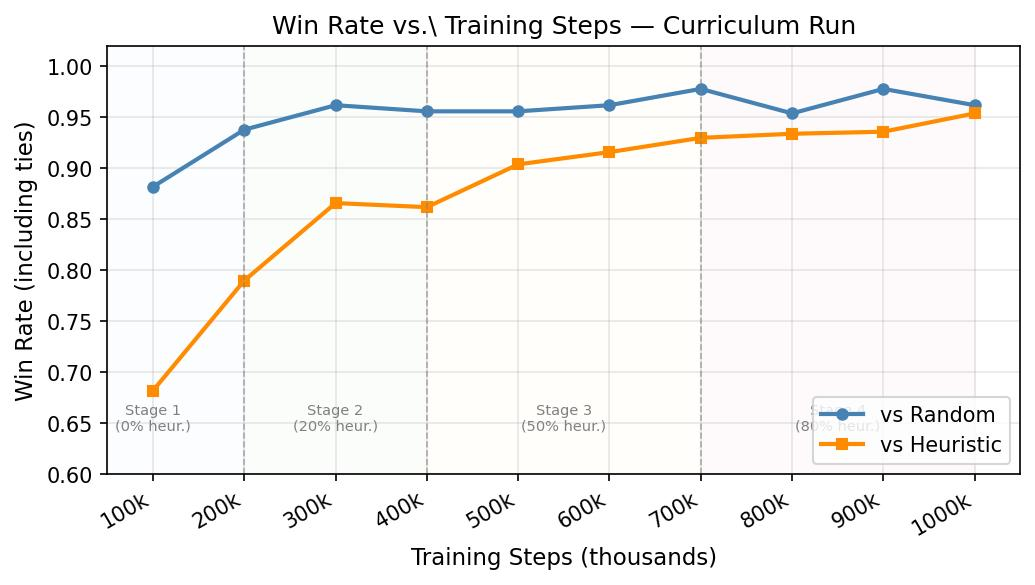
\includegraphics[width=0.85\textwidth]{winrate_vs_steps.jpg}
  \caption{Win rate (including ties) versus training steps for the reproduced curriculum run. Shaded bands indicate the four curriculum stages: Stage~1 (0\% heuristic, 0--200k steps), Stage~2 (20\%, 200--400k), Stage~3 (50\%, 400--700k), Stage~4 (80\%, 700k--1M). Each point is 500 deterministic evaluation episodes.}
  \label{fig:winrate-vs-steps}
\end{figure}

Performance against random opponents rises quickly in Stage~1, reaching 0.938 by 200k steps, and then plateaus around 0.96--0.98 from 300k onward. Performance against the heuristic baseline improves more gradually and continues to rise throughout Stage~3 and Stage~4 as heuristic exposure increases, reaching 0.954 at 1M steps. The gap between the two curves closes steadily across the later curriculum stages, which is consistent with the hypothesis that increasing heuristic pressure in later stages is the main driver of policy improvement against structured opponents.

\subsection{Ablation: opponent training regime}
\label{sec:ablation}

To quantify the benefit of curriculum training, two ablation runs were trained under identical hyperparameters and seed for 1M steps but with a fixed single-opponent regime throughout: one trained against the random agent only (\textit{random-only}) and one trained against the heuristic agent only (\textit{heuristic-only}). Table~\ref{tab:ablation} reports deterministic 1000-episode evaluation results for all three conditions.

\begin{table}[H]
\centering
\begin{tabularx}{\textwidth}{@{}lcccc@{}}
\toprule
Training regime & vs Random win rate & vs Random score diff & vs Heuristic win rate & vs Heuristic score diff \\
\midrule
Random-only     & 0.968 & +18.057 & 0.866 & +12.376 \\
Heuristic-only  & 0.955 & +16.318 & 0.955 & +16.360 \\
Curriculum      & 0.966                     & +17.573                   & 0.957                     & +16.238                  \\
\bottomrule
\end{tabularx}
\caption{Ablation: 1000-episode deterministic evaluation for three training regimes at 1M steps. All runs use seed~1 for ablation conditions and seed~0 for the curriculum run.}
\label{tab:ablation}
\end{table}

The results support the following conclusions. Training against random opponents only produces the highest win rate against random play (0.968) but a noticeably weaker win rate against the heuristic (0.866), indicating that the policy overfits to exploiting random behaviour and does not generalise to structured opponents. Training against the heuristic opponent only produces balanced results: 0.955 against both random and heuristic, at the cost of a slightly lower score margin against random (+16.318 vs +18.057). The curriculum condition achieves a strong win rate against both opponents (0.966 vs random, 0.957 vs heuristic) and score margins comparable to or exceeding the single-regime alternatives in both evaluation matchups. Taken together, the ablation confirms that curriculum training provides the most robust generalisation across opponent types, with neither the random-only bias nor the reduced random-exploitation of the heuristic-only condition.

\subsection{Qualitative LLM interaction examples}

To show how the auxiliary explain and coach layer communicates with a player, this report includes short extracts from the saved transcript \texttt{runs/llm\_logs/llm\_demo\_20260326\_191704.txt}. That transcript used the Gemini provider (\texttt{gemini-2.5-flash}) with the reproduced RL policy, and the sampled game ended in a 62--40 win for the agent.

The first example shows opening-turn coaching. The assistant turns the policy ranking into direct tactical advice:
\begin{quote}\small
``Scores 3 immediate points, which is the highest individual card score available in the current hand. Tradeoff: Does not contribute to set collection for bonus points (like Tempura or Sashimi) or save a high-value Nigiri for a potential Wasabi multiplier.''
\end{quote}

The second example shows an explanation of a chopsticks double-play:
\begin{quote}\small
``It completes a set of three sashimi, securing 10 points. Given only 3 cards left this turn, securing this significant score is critical. Tradeoff: An alternative is playing the tempura, which would complete a pair for 5 points.''
\end{quote}

The third example shows that the assistant can also verbalise defensive reasoning:
\begin{quote}\small
``Playing tempura increases your count to 3, but critically, it denies the opponent the card they need to complete a pair and score 5 points this round.''
\end{quote}

These examples do not prove that the LLM layer is pedagogically optimal, but they do show that the repository already supports a grounded coaching workflow in which policy probabilities, visible game state, and natural-language explanation are preserved together in one transcript artifact.

\section{Discussion}

The experiments support four main conclusions.

First, the environment is learnable. The reproduced model comfortably outperforms both random play and the heuristic baseline, which shows that the reward, state encoding, and action masking are sufficient for strong policy learning.

Second, opponent diversity matters. The ablation study (Section~\ref{sec:ablation}) directly quantifies this: training against random opponents only yields a win rate of 0.866 against the heuristic (a 9-point drop from the curriculum's 0.957), while training against the heuristic only yields 0.955 against both opponents but sacrifices some win margin against random play. The curriculum achieves the strongest generalisation across both matchups simultaneously, confirming that progressive opponent mixing is the key driver of robustness rather than simply training against a harder fixed opponent for longer.

Third, the project is in a much better reproducibility state when the reported best model is a checkpoint trained directly from the current scripts with preserved command lines and matching evaluation notes.

Fourth, the LLM interface is meaningful precisely because the policy underneath it is strong. If the underlying agent were weak, fluent explanations would have little value. Here, the qualitative transcript examples are more convincing because they are attached to a policy that already demonstrates strong quantitative performance.

There are still clear limitations. The reproduced model is strong under the chosen curriculum and seed, but this report does not quantify variance across many independent training seeds. Evaluation focuses on scripted baselines rather than human players. The game remains a constrained Sushi Go variant with two players and a fixed three-round format. The LLM explain and coach component improves usability and interpretability, but it has not yet been evaluated for actual human usefulness beyond repository tooling support. Finally, LLM output quality is provider-dependent: the grounding data are stable, but the exact wording varies between Gemini, OpenAI, and fallback template modes.

The most useful next steps are to preserve training metadata automatically for every checkpoint, run multiple 1M-step seeds and report variance across seeds, and evaluate whether the LLM coach actually helps human decision making in interactive play.

\section{Conclusion}

This project successfully implements a deterministic, rule-correct, and testable Sushi Go reinforcement learning system. The environment design is technically coherent: scoring is isolated in pure functions, legal-action masking is explicit, and seeded determinism is built into the simulation. The baseline controls behave as expected, the reproducibility check passes, and the full test suite succeeds.

Most importantly, the merged report now demonstrates empirical performance rather than only describing an architecture. A fresh 1,000,000-step curriculum training run from the current repository produces \texttt{repro\_curriculum\_1m}, which achieves 96.6\% win rate against random play and 95.7\% against the heuristic baseline over 1000 deterministic episodes. That result supports the central claim of the project: a masked PPO policy can learn a strong strategy in this constrained, sparse-reward Sushi Go environment, and the current codebase can reproduce that result directly. Furthermore, the ablation study demonstrates that curriculum training is specifically responsible for this generalisation: a policy trained against random opponents only achieves only 0.866 against the heuristic, while the curriculum policy achieves 0.957, confirming that progressive opponent mixing rather than sheer training volume explains the robustness of the final model. The qualitative transcript extracts also show that the optional LLM layer can present that learned strategy to a human player in grounded, state-aware language rather than opaque action indices alone.

\appendix
\section{Appendix}

\subsection{Reproducibility commands}

The following commands were used to produce the main numbers reported in this document from the repository root:

\begin{verbatim}
conda run -n sushigo-rl env PYTHONPATH=src python -m pytest -q

conda run -n sushigo-rl env PYTHONPATH=src MPLCONFIGDIR=/tmp/matplotlib \
python -m sushigo_rl.eval --opponents none --baselines random_vs_random \
  --episodes 1000

conda run -n sushigo-rl env PYTHONPATH=src MPLCONFIGDIR=/tmp/matplotlib \
python -m sushigo_rl.eval --opponents none --baselines heuristic_vs_random \
  --episodes 1000

conda run -n sushigo-rl env PYTHONPATH=src MPLCONFIGDIR=/tmp/matplotlib \
python -m sushigo_rl.eval --opponents none --baselines none --repro-check \
  --repro-seed 17

PYTHONPATH=src /home/simon/miniconda3/envs/sushigo-rl/bin/python \
  -m sushigo_rl.train --opponent-mode curriculum \
  --curriculum-stages "0.0:200000,0.2:200000,0.5:300000,0.8:300000" \
  --timesteps 1000000 --seed 0 --vecnorm \
  --vecnorm-path runs/repro_curriculum_1m.vecnormalize.pkl \
  --model-out runs/repro_curriculum_1m --checkpoint-every 100000 \
  --checkpoint-dir runs/repro_curriculum_1m_checkpoints \
  --checkpoint-prefix model --verbose 0

conda run -n sushigo-rl env PYTHONPATH=src MPLCONFIGDIR=/tmp/matplotlib \
python -m sushigo_rl.eval --model runs/repro_curriculum_1m.zip \
  --vecnorm-path runs/repro_curriculum_1m.vecnormalize.pkl \
  --episodes 1000 --opponents both --baselines none --deterministic

# Ablation: random-only training
PYTHONPATH=src /home/simon/miniconda3/envs/sushigo-rl/bin/python \
  -m sushigo_rl.train --opponent-mode random \
  --timesteps 1000000 --seed 1 --vecnorm \
  --vecnorm-path runs/ablation_random_only.vecnormalize.pkl \
  --model-out runs/ablation_random_only --verbose 0

# Ablation: heuristic-only training
PYTHONPATH=src /home/simon/miniconda3/envs/sushigo-rl/bin/python \
  -m sushigo_rl.train --opponent-mode heuristic \
  --timesteps 1000000 --seed 1 --vecnorm \
  --vecnorm-path runs/ablation_heuristic_only.vecnormalize.pkl \
  --model-out runs/ablation_heuristic_only --verbose 0

conda run -n sushigo-rl env PYTHONPATH=src MPLCONFIGDIR=/tmp/matplotlib \
python -m sushigo_rl.eval --model runs/ablation_random_only.zip \
  --vecnorm-path runs/ablation_random_only.vecnormalize.pkl \
  --episodes 1000 --opponents both --baselines none --deterministic

conda run -n sushigo-rl env PYTHONPATH=src MPLCONFIGDIR=/tmp/matplotlib \
python -m sushigo_rl.eval --model runs/ablation_heuristic_only.zip \
  --vecnorm-path runs/ablation_heuristic_only.vecnormalize.pkl \
  --episodes 1000 --opponents both --baselines none --deterministic
\end{verbatim}

\subsection{Checkpoint performance table}

Table~\ref{tab:checkpoint-perf} reports the win rate and mean score difference at each 100k-step checkpoint from the curriculum run, evaluated deterministically over 500 episodes per opponent. These are the underlying data points plotted in Fig~\ref{fig:winrate-vs-steps}.

\begin{table}[H]
\centering
\begin{tabularx}{\textwidth}{@{}rcccc@{}}
\toprule
Steps & vs Random WR & vs Random score diff & vs Heuristic WR & vs Heuristic score diff \\
\midrule
100k  & 0.882 & +11.792 & 0.682 & +5.752  \\
200k  & 0.938 & +14.082 & 0.790 & +8.224  \\
300k  & 0.962 & +16.526 & 0.866 & +11.054 \\
400k  & 0.956 & +16.318 & 0.862 & +11.514 \\
500k  & 0.956 & +17.250 & 0.904 & +12.656 \\
600k  & 0.962 & +17.164 & 0.916 & +13.470 \\
700k  & 0.978 & +17.522 & 0.930 & +14.818 \\
800k  & 0.954 & +17.066 & 0.934 & +14.876 \\
900k  & 0.978 & +18.070 & 0.936 & +15.618 \\
1000k & 0.962 & +17.774 & 0.954 & +15.728 \\
\bottomrule
\end{tabularx}
\caption{Win rate (including ties) and mean score difference at each checkpoint of the curriculum run, evaluated over 500 deterministic episodes per opponent. WR = win rate including ties.}
\label{tab:checkpoint-perf}
\end{table}

\end{document}
